\chapter{Аналитический раздел}

\section{Управление памятью в операционной системе}

Для хранения данных запущенных в операционной системе процессов, находящихся в состоянии выполнения, ожидания или блокировки, используется оперативная память. Устройство, предназначенное для записи, считывания и хранения инструкций и данных процессов, называется оперативным запоминающим устройством (ОЗУ) \cite{ram}. В многозадачных системах память должна быть распределена для размещения нескольких процессов. Для управления памятью в системе используется абстракция адресного пространства. У каждого процесса имеется собственное адресное пространство --- набор адресов, который может быть использован процессом для обращения к памяти \cite{address-space}. Если объем оперативной памяти, необходимый для размещения данных всех процессов, превышает объем ОЗУ, то возникает перегрузка памяти. Одним из способов решения проблемы является виртуальная память.

\subsection{Виртуальная память}

Механизм виртуальной памяти предполагает разделение логической памяти и физической памяти. У каждого процесса имеется собственное виртуальное адресное пространство. При использовании страничной организации памяти, виртуальное адресное пространство делится на блоки фиксированного размера, называемые страницами. Физическая память делится на блоки байт фиксированного размера, называемые страничным блоком или кадром. Страницы виртуального адресного пространства и страничные блоки имеют одинаковый размер, который определяется аппаратным обеспечением. Значение размера представляет собой степень двойки и изменяется от четырех килобайт до одного гигабайта \cite{swapping}.

При использовании виртуальной памяти процессы оперируют виртуальными адресами. Виртуальный адрес --- это адрес, присвоенный местоположению в виртуальной памяти, который позволяет обращаться к данному местоположению так, как если бы это была часть физической памяти \cite{address-space}. Отображение виртуального адреса на физический адрес памяти выполняется диспетчером памяти с использованием таблиц страниц, как показано на рисунке \ref{img:virtual-memory}.

\includeimage
    {virtual-memory}
    {f}
    {h}
    {0.9\textwidth}
    {Схема работы виртуальной памяти}
    
Одним из основных преимуществ использования виртуальной памяти является то, что объем памяти, размещающий данные процессов не ограничен объемом доступной физической памяти. В системах с виртуальной памятью используется подкачка страниц по запросу.

\subsection{Подкачка страниц}

Данные процесса или их часть можно выгружать из оперативной памяти в резервное хранилище, а затем возвращать в память для продолжения выполнения. Резервное хранилище представляет собой вторичное хранилище, разделенное на блоки фиксированного размера, которые имеют тот же размер, что и страничные кадры. Таким образом, неиспользуемая страница памяти может быть перемещена в резервное хранилище, и загружена в оперативную память при необходимости. Этот принцип работы получил название подкачка страниц, при этом вторичное хранилище называется устройством подкачки, а его раздел, используемый для хранения данных --- пространством подкачки~\cite{swapping}.

Присутствие страницы в оперативной памяти отслеживается с помощью бита присутствия-отсутствия \cite{address-space}. Если процесс попытается получить доступ к отсутствующей в памяти странице, возникает системное прерывание (page fault). Операционная система находит свободный страничный кадр или выбирает редко используемую страницу и сбрасывает ее содержимое во вторичное хранилище. Затем она перемещает нужную физическую страницу в свободный страничный кадр. Схема работы подкачки страниц при возникновении page fault приведена на рисунке \ref{img:demand-paging}.

\includeimage
    {demand-paging}
    {f}
    {h}
    {0.9\textwidth}
    {Схема работы подкачки страниц при возникновении page fault}
    
Подкачка страниц позволяет загружать только требуемые для выполнения данные, но для переноса страниц между вторичным хранилищем и оперативной памятью требуется время. Частое перемещение снижает производительность работы подсистемы памяти. Для решения этой проблемы используется сжатие памяти \cite{swapping-problem}.

\section{Сжатие данных}\label{compression}

Неслучайные данные имеют некоторую структуру. Наличие у данных структуры, которую можно использовать для уменьшения их размера путем достижения такого представления данных, в котором никакая структура не выделяется, называют избыточностью. Сжатие данных --- это процесс преобразования исходных данных в их компактную форму путем распознавания и использования избыточности данных \cite{compression-definition}. Процесс сжатия состоит из двух этапов:

\begin{enumerate}
	\item Этап моделирования, который включает в себя распознавание избыточности для построения модели. Модель представляет собой набор данных и правил, используемых для обработки входных символов.
	\item Этап кодирования данных с использованием модели.
\end{enumerate}

Описанные этапы сжатия данных представлены на рисунке \ref{img:compression-steps}.

\includeimage
    {compression-steps}
    {f}
    {h}
    {0.6\textwidth}
    {Этапы сжатия данных}

В результате сжатия исходных данных $X$ получается их представление~$X_{\text{сж}}$. При восстановлении сжатые данные $X_{\text{сж}}$ преобразуются в представление~$Y$. На основании требований к восстановлению выделяют \cite{compression-classes}:

\begin{itemize}
	\item сжатие данных без потерь, при котором $Y = X$;
	\item сжатие данных с потерями, при котором $Y \not= X$.
\end{itemize}

Схемы сжатия данных без потерь и с потерями показаны на рисунке \ref{img:compression-classes}.

\includeimage
    {compression-classes}
    {f}
    {h}
    {0.8\textwidth}
    {Схемы сжатия данных без потерь и с потерями}

\subsection{Сжатие памяти}

Сжатие памяти заключается в том, что несколько страничных кадров сжимаются, их сжатые версии сохраняются в меньшем числе страничных кадров. Это позволяет системе сократить использование памяти, не прибегая к подкачке страниц. Если процессу требуются сжатые страницы, они восстанавливаются~\cite{swapping}.

На рисунке \ref{img:memory-compression} приведена схема сжатия памяти: неиспользуемые страницы 2-5 хранятся в сжатом виде, в результате увеличивается объем свободной памяти.

\includeimage
    {memory-compression}
    {f}
    {h}
    {0.8\textwidth}
    {Схема сжатия памяти}

Выделяют следующие требования к реализации сжатия памяти~\cite{compression-requirements}:

\begin{itemize}
	\item при запросе на чтение данные должны восстанавливаться без потерь;
	\item операции сжатия и восстановления должны иметь низкую временную задержку и высокую производительность.
\end{itemize}

\subsection{Коэффициент сжатия}

Для измерения производительности сжатия используют характеристику, которую называют коэффициентом сжатия и определяют следующим образом~\cite{compression-coefficient}:

\begin{equation}\label{compression-coefficient}
	K_{\text{сж}} = \frac{L_{\text{исх}}}{L_{\text{сж}}},
\end{equation}

\noindentгде $L_{\text{исх}}$ --- объем исходных данных, $L_{\text{сж}}$ --- объем сжатых данных.

TODO: описать другие метрики производительности сжатия

Из формулы (\ref{compression-coefficient}) видно, что если размер сжатых данных близок к размеру исходных данных, то коэффициент сжатия будет близок к единице. Коэффициент сжатия меньше единицы в случае, если размер полученных после сжатия данных больше размера исходных данных.

Использование методов сжатия с потерями приводит к большему коэффициенту сжатия, но часть исходных данных теряется при восстановлении \cite{compression-definition}. Выбор алгоритма сжатия зависит от условий задачи, для решения которой применяется сжатие. При этом, стремятся увеличить скорость и коэффициент сжатия. Оценить коэффициент сжатия можно с помощью информационной энтропии.

\section{Информационная энтропия}\label{ientropy}

Под информацией понимают сведения, которые являются объектом хранения, передачи и обработки \cite{information}. Формой представления информации является сообщение. Физическую величину, отображающую сообщение, называют сигналом. Передача информации осуществляется следующим образом~\cite{transmission}:

\begin{enumerate}
	\item Источник информации создает случайное сообщение. В теории информации любой источник информации является стохастическим, его можно описать измеряемыми вероятностными категориям.
	\item Сообщение поступает в систему передачи, в которой выполняется кодирование --- преобразование сообщения c целью согласования источника информации с каналом связи для увеличения скорости передачи информации или обеспечения заданной помехоустойчивости  \cite{information}. Кодирование состоит из шифрования, сжатия и защиты от шума, в результате которых формируется сигнал. 
	\item Сигнал проходит через канал --- среду передачи информации \cite{transmission}. В канале могут возникать помехи, создаваемые источником шума.
	\item Сигнал подается на вход системе приема, которая выполняет декодирование --- восстановление исходного сообщения \cite{information}.
	\item Исходное сообщение передается получателю.
\end{enumerate}

Описанная схема передачи информации представлена на рисунке \ref{img:transmission}.

\includeimage
    {transmission}
    {f}
    {h}
    {1\textwidth}
    {Схема передачи информации}
    
Сообщение содержит сведения о некоторой физической системе $X$, которая случайным образом может перейти в какое-либо состояние $x_{i}$ из конечного множества состояний $x_{1}, x_{2}, \dots, x_{n}$ c вероятностями $p_{1}, p_{2}, \dots, p_{n}$, где $n \in \mathbb{N}$, $p_{i} = P(X \sim x_{i})$ и $\sum_{i = 1}^n p_{i} = 1$. То есть, для такой системы существует степень неопределенности, которая описывается числом ее возможных состояний и их вероятностями. Сведения из принятого сообщения тем ценнее, чем больше была неопределенность системы до получения сообщения. Специальную характеристику, используемую в качестве меры неопределенности системы, называют информационной энтропией \cite{definition}. Информационная энтропия конечной вероятностной схемы определяется по формуле Шеннона:

\begin{equation}\label{entropy}
	H(X) = -\sum_{i = 1}^n (p_{i} \cdot \log_{a}p_{i}),
\end{equation}

\noindentгде $p_{i} \in [0, 1]$, $a > 1$.

Основание логарифма определяет единицы измерения информационной энтропии: при $a = 2$ энтропия измеряется в битах, при $a = 3$ --- в тритах, при $a = e$ --- в натах.

\subsection{Свойства информационной энтропии}\label{properties}

Информационная энтропия обладает следующими свойствами \cite{properties}:

\begin{enumerate}
	\item Энтропия всегда неотрицательна. Значения $\log_{a} p_{i}$ в формуле (\ref{entropy}) принимают неположительные значения, так как $p_{i} \in [0, 1]$. Поэтому
	
\begin{equation}
	H(X) = -\sum_{i = 1}^n (p_{i} \cdot \log_{a} p_{i}) \geqslant 0.
\end{equation}

	\item\label{property2} Энтропия равна нулю, если состояние системы в точности известно заранее. Если известно состояние $x_{k}$, в которое перейдет система $X$, то вероятность этого состояния $p_{k}$ равна единице, вероятности других состояний равны нулю. Тогда
	
\begin{equation}
	p_{k} \cdot \log_{a} p_{k} = 1 \cdot \log_{a} 1 = 1 \cdot 0 = 0.
\end{equation}

В связи с тем, что $\lim\limits_{p \to 0} (p \cdot \log_{a}p) = 0$, другие слагаемые суммы в формуле~(\ref{entropy}) равны нулю. В этом случае 

\begin{equation}
	H(X) = -\sum_{i = 1}^n (p_{i} \cdot \log_{a} p_{i}) = 0.
\end{equation}

	\item\label{property3} Энтропия принимает наибольшее значение при условии, что все состояния равновероятны, то есть, $p_{1} = p_{2} = \dots = p_{n} = \frac{1}{n}$. Тогда
	
\begin{equation}
	H(X) = -\sum_{i = 1}^n (p_{i} \cdot \log_{a} p_{i}) = -\sum_{i = 1}^n (\frac{1}{n} \cdot \log_{a} \frac{1}{n}) = -\log_{a} \frac{1}{n} = \log_{a} n.
\end{equation}
	
\end{enumerate}

\subsection{Связь с коэффициентом сжатия}\label{relation}

Данные, обладающие предсказуемой структурой, сокращают неопределенность системы меньше, чем сведения, в которых никакая структура не выделяется. Так как информационная энтропия является мерой неопределенности системы, то данные с выделяемой структурой, имеют низкое значение энтропии. Сведения, в которых закономерности не определяются, имеют высокое значение энтропии \cite{relation}. Так, чем меньше избыточность данных, тем выше значение их энтропии. То есть, информационная энтропия сжатых данных выше, чем ее значение до сжатия.

Согласно теореме Шеннона об источнике шифрования сигнал, обладающий размером $S$ и информационной энтропией $H$, не может быть сжат менее, чем до $S \cdot H$ битов без потери точности информации. Таким образом, на основании информационной энтропии исходных данных определяется теоретическая граница коэффициента сжатия \cite{theorem}.

В связи с применением операций сложения, умножения и логарифмирования при вычислении энтропии по формуле (\ref{entropy}), число которых растет с увеличением объема данных, встает задача выбора метода подсчета. Использование метода влияет на скорость и время определения информационной энтропии.

\section{Методы подсчета информационной энтропии}

\subsection{Метод скользящего окна}\label{sliding-window}

При решении задач, связанных со сжатием, данные $X$ представляют собой массив байтов размером $N$ \cite{bytes}. Байт состоит из восьми битов, каждый из которых кодирует одно из значений множества $\{0, 1\}$. Поэтому один байт может принимать значения из интервала от 0 до 255 включительно в десятичной системе счисления. 

В методе скользящего окна под окном понимают рассматриваемую на текущем этапе подпоследовательность данных размером $n$ \cite{sliding-window-method}. При подсчете энтропии данным методом необходима дополнительная память размером $2^n$ для хранения числа вхождений подпоследовательностей данных. Так как с увеличением размера окна, растет объем дополнительной памяти, в качестве окна выбирается минимально адресуемая единица памяти, которой является байт \cite{memory-unit}. В связи с тем, что на каждом этапе окно смещается на следующие восемь битов, как показано на рисунке \ref{img:sliding-window}, оно называется скользящим.

\includeimage
    {sliding-window}
    {f}
    {h}
    {1\textwidth}
    {Проход по массиву байтов методом скользящего окна}
    
Вычисление информационной энтропии методом скользящего окна включает в себя два шага:

\begin{enumerate}
	\item Для каждого возможного значения байта подсчитывается число его вхождений $k_{i}$ в массив байтов, где $i = \overline{0, 255}$.
	\item С учетом того, что вероятность появления байта в массиве $p_{i} = \frac{k_{i}}{N}$, информационная энтропия вычисляется по следующей формуле:
	
	\begin{equation}
		H(X) = -\sum_{i = 0}^{255} (p_{i} \cdot \log_{2}p_{i}).
	\end{equation}
\end{enumerate}

Так как первый шаг метода предполагает проход по массиву байтов размером $N$, а второй шаг --- проход по массиву числа вхождений подпоследовательностей данных размером $2^n$, временная сложность метода скользящего окна --- $O(N + 2^n)$. 

Информационная энтропия, подсчитанная методом скользящего окна, принимает значения из интервала $[0, 8]$ битов. При этом согласно свойству~\ref{property2} из подраздела \ref{properties} информационная энтропия принимает нулевое значение в случае, когда массив данных состоит из одинаковых байтов, и в соответствии со свойством~\ref{property3} из подраздела \ref{properties} максимальное значение, равное восьми, если все байты в массиве различны.

\subsection{Биномиальный метод}\label{binomial}

В биномиальном методе вычисления информационной энтропии \cite{binomial-method} данные~$X$ рассматриваются как последовательность сообщений, генерируемых бернуллиевским источником --- источником информации, порождающим символы из алфавита $\{0; 1\}$ с вероятностями $1 - p$ и $p$ соответственно, причем $p \in (0, 1)$ и может быть неизвестно \cite{bernullie-source}. То есть, сообщение представляет собой последовательность битов длины $n$.

Вероятность того, что сообщение содержит $k$ единиц, где $k = \overline{0, n}$, вычисляется следующим образом:

\begin{equation}\label{pk}
	P_{k} = p^k \cdot (1 - p)^{(n - k)}.
\end{equation} 

Количество возможных сообщений, содержащих $k$ единиц, определяется как биномиальный коэффициент:

\begin{equation}\label{binomial-coefficient}
	C_{n}^k = \frac{n!}{k! \cdot (n - k)!}.
\end{equation}

В связи с тем, что $k$ может принимать значения из интервала $[0, n]$, число биномиальных коэффициентов, подсчитанных по формуле (\ref{binomial-coefficient}), равно $n + 1$. Это означает, что сообщения можно разбить на $n + 1$ классов эквивалентности. Тогда информационная энтропия вычисляется так:

\begin{equation}\label{binomial-entropy}
	H(X) = -\sum_{k = 0}^n (C_{n}^k \cdot P_{k} \cdot \log_{2}P_{k}).
\end{equation}

В соответствии с формулой (\ref{binomial-entropy}) биномиальный метод подсчета информационной энтропии состоит из следующих этапов:

\begin{enumerate}
	\item Исходные сообщения разбиваются на $n + 1$ классов эквивалентности, сообщения которых содержат $k = \overline{0, n}$ единиц.
	\item Для каждого класса эквивалентности рассчитывается биномиальный коэффициент~$C_{n}^k$.
	\item Определяются вероятности $p$ появления единицы в сообщениях.
	\item Вычисляются вероятности $P_{k}$ по формуле (\ref{pk}).
	\item Суммируются произведения биномиальных коэффициентов $C_{n}^k$, вероятностей $P_{k}$ и логарифмов вероятностей $P_{k}$ для всех $n + 1$ значений~$k$.
\end{enumerate}

Схема определения биномиальных коэффициентов $C_{n}^k$ и вероятностей~$P_{k}$ приведена на рисунке \ref{img:binomial-method}.

\includeimage
    {binomial-method}
    {f}
    {h}
    {0.9\textwidth}
    {Определение биномиальных коэффициентов $C_{n}^k$ и вероятностей~$P_{k}$}

Для определения вероятности $p$ появления единицы в сообщениях на третьем этапе биномиального метода необходима дополнительная память размером $n + 1$. При этом данный этап подразумевает проход по массиву байтов размером $N$. Последний этап вычисления предполагает проход по массиву, содержащему значения вероятностей $p$ появления единицы в сообщениях. Тогда временная сложность биномиального метода подсчета информационной энтропии --- $O(N + n)$.

В биномиальном методе определяются вероятности появления не подпоследовательности, а единицы в подпоследовательностях. Кроме того, расчет ускоряется за счет разделения исходной последовательности на классы эквивалентности, что приводит к сокращению операций сложения.

При рассмотрении бернуллиевского источника информации предполагается, что вероятность появления единицы в подпоследовательности не зависит от вероятностей появления нуля или единицы в битах предыдущей подпоследовательности. При наличии такой зависимости вычисленное значение энтропии будет завышено. Так как рассматриваемое представление данных --- последовательность битов, то вероятности появления каждого значения бита независимы. 

Недостатком данного метода является трудоемкость вычисления факториала при определении биномиальных коэффициентов с увеличением длины подпоследовательности. Для снижения времени подсчета биномиальных коэффициентов можно хранить их значения в дополнительном массиве. Так как для сообщения длины $n$ количество требуемых для определения энтропии биномиальных коэффициентов равно $n + 1$, то для их хранения потребуется память размером $n + 1$.

\subsection{Сравнение существующих методов подсчета}

При вычислении информационной энтропии методом скользящего окна и биномиальным методом операции сложения, умножения и логарифмирования применяются к целым числам и числам с плавающей запятой.

Для сравнения методов подсчета информационной энтропии были выделены следующие критерии оценки:

\begin{itemize}
	\item K1 --- временная сложность;
	\item K2 --- необходимость вычисления факториала;
	\item K3 --- возможность распараллеливания вычислений;
	\item K4 --- объем требуемой дополнительной памяти.
\end{itemize}

Результаты сравнения представлены в таблице \ref{tab:comparison}.

\begin{table}[h]
    \caption{Сравнение методов подсчета информационной энтропии}
    \begin{center}
        \begin{tabular}{|l|l|l|l|l|}
        		\hline
            \multicolumn{1}{|c}{\textbf{Метод}} & 
            \multicolumn{1}{|c|}{\textbf{K1}} &
            \multicolumn{1}{c|}{\textbf{K2}} &
            \multicolumn{1}{c|}{\textbf{K3}} & 
            \multicolumn{1}{c|}{\textbf{K4}} \\ \hline
            Скользящего окна &  $O(N + 2^n)$ & $-$ & $+$ & $2^n$ \\ \hline
            Биномиальный &  $O(N + n)$ & $+$ & $+$ & $2 \cdot (n + 1)$ \\ \hline
        \end{tabular}
    \end{center}
    \label{tab:comparison}
\end{table}

Таким образом, биномиальный метод подсчета информационной энтропии требует меньших вычислительных затрат по времени и по памяти.

\section{Постановка задачи}

Из проведенного в разделах \ref{compression}-\ref{ientropy} анализа сжатия и информационной энтропии можно сделать следующие выводы:

\begin{itemize}
	\item сжатие и восстановление страниц оперативной памяти должно иметь низкую временную задержку и высокий коэффициент сжатия;
    \item коэффициент сжатия принимает низкое значение, если размер сжатых данных близок к размеру исходных данных или превышает его;
	\item значение информационной энтропии исходных данных позволяет определить теоретическую границу коэффициента сжатия.
\end{itemize}

Так, сжатие может иметь низкую производительность, при этом на него будет тратиться время. Можно сократить временные затраты на сжатие, если определять коэффициент сжатия до его выполнения, и на основании оценки производительности принимать решение, сжимать страницу или нет. Производительность сжатия по исходным данным можно оценить с помощью информационной энтропии. Таким образом, необходимо провести оптимизацию сжатия страниц памяти, принимая решение о его выполнении на основании вычисленного значения информационной энтропии исходных данных.

Входными данными поставленной задачи является страница памяти, которая представляет собой вектор $a = (a_1\text{ }a_2\text{ }\dotso\text{ }a_N)$ размером $N$, равным размеру страницы памяти. При этом, $0 \leq a_i \leq 255$.

На принятие решения о выполнении сжатия влияет сравнение подсчитанного значения информационной энтропии с пороговым значением. Сжатие страниц памяти выполняется ядром операционной системы.

В зависимости от принятого решения выходными данными могут быть:
\begin{itemize}
	\item страница памяти со сжатыми исходными данными, которая представляет собой вектор $b = (b_1\text{ }b_2\text{ }\dotso\text{ }b_N)$ размером $N$, $0 \leq b_i \leq 255$;
    \item страница памяти с исходными данными, которая представляет собой вектор $a$.
\end{itemize}

На рисунке \ref{img:zero-level} показана IDEF0-диаграмма нулевого уровня, формализующая поставленную задачу.

\begin{figure}[H]
	\begin{center}
		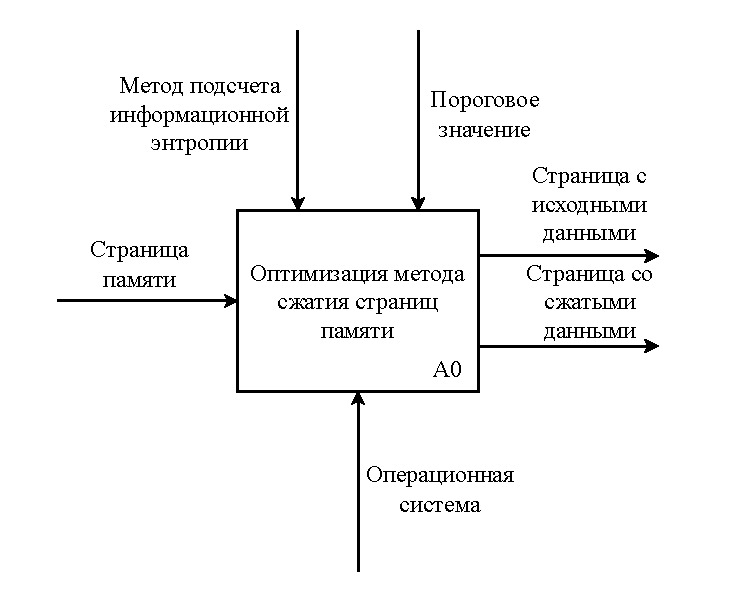
\includegraphics[scale=0.7]{inc/img/zero-level.pdf}
	\end{center}
	\captionsetup{justification=centering}
	\caption{IDEF0-диаграмма нулевого уровня}
	\label{img:zero-level}
\end{figure}

\section{Сравнение операционных систем}

Выполнение оптимизации метода сжатия страниц памяти должно проводиться на операционной системе, удовлетворяющей следующим критериям:

\begin{itemize}
	\item поддержка сжатия страниц оперативной памяти;
	\item открытый исходный код.
\end{itemize}

Для сравнения, приведенного в таблице \ref{tab:comparison-os}, были выбраны системы, занимающие наибольшие доли рынка операционных систем \cite{stat}.

\begin{table}[h]
    \caption{Сравнение операционных систем}
    \begin{center}
        \begin{tabular}{|l|l|l|l|}
        		\hline
            \multicolumn{1}{|c}{\textbf{Операционная}} & 
            \multicolumn{1}{|c|}{\textbf{Поддержка}} &
            \multicolumn{1}{c|}{\textbf{Открытый}} &
            \multicolumn{1}{c|}{\textbf{Доля}} \\
            \multicolumn{1}{|c}{\textbf{система}} & 
            \multicolumn{1}{|c|}{\textbf{сжатия}} &
            \multicolumn{1}{c|}{\textbf{исходный код}} &
            \multicolumn{1}{c|}{\textbf{рынка (\%)}} \\ \hline
            Windows &  + & - & 63.13 \\ \hline
            OS X & + & - & 17.78 \\ \hline
            Linux & + & + & 2.83 \\ \hline
            FreeBSD & + & + & 0.01 \\ \hline
        \end{tabular}
    \end{center}
    \label{tab:comparison-os}
\end{table}

В дальнейшем будет рассматриваться ядро операционной системы Linux, так как она удовлетворяет выделенным критериям и занимает долю рынка большую, чем операционная система FreeBSD.

\section{Сжатие памяти в ядре Linux}

Ядро Linux является модульным. Модуль --- это часть кода, которую можно загрузить и выгрузить в ядро по необходимости \cite{module}. Модуль может быть встроенным или загружаемым.

Код встроенного модуля встраивается в образ ядра во время компиляции. Если ядру потребуется функциональность этого модуля, оно инициализирует и загрузит модуль. Для того, чтобы изменения такого модуля вступили в силу, необходимо перекомпилировать ядро.

Загружаемый модуль может быть загружен пользователем в ядро во время работы системы. Такие модули используют для добавления требуемой функциональности ядра без перезагрузки системы. Это позволяет избежать пересборки и перезагрузки ядра при каждом добавлении новых функций. 

Возможность сжатия страниц оперативной памяти в ядре Linux предоставляют загружаемые модули zram и zswap.

\subsection{Модуль zram}

При загрузке модуля zram в оперативной памяти создается блочный специальный файл. Специальные файлы в операционной системе Linux служат для реализации работы с устройствами ввода-вывода как с файлами и находятся в каталоге /dev. Это позволяет драйверам устройств проводить с устройствами ввода-вывода операции чтения и записи, используя те же системные
вызовы, которые применяются для чтения и записи файлов. Блочные специальные файлы используются для моделирования устройств, содержащих набор блоков с произвольной адресацией. Открыв такой файл, программа может получить доступ к любому блоку устройства независимо от структуры имеющейся файловой системы \cite{block-file}. При этом данные могут быть прочитаны или записаны только кратными блоками.

Созданный модулем zram блочный специальный файл моделирует диск. После загрузки модуля страницы, попадаемые на вход моделируемому диску, сжимаются и хранятся сжатыми. Таким образом, страницы находятся в оперативной памяти в сжатом виде.

На рисунке \ref{img:zram} представлена схема работы модуля zram.

\includeimage
    {zram}
    {f}
    {h}
    {0.7\textwidth}
    {Схема работы модуля zram}

Модуль zram дает следующие преимущества \cite{zram}:

\begin{itemize}
	\item сокращение использования памяти за счет сжатия страниц;
	\item высокая скорость операций чтения и записи, так как блочный специальный файл создается в оперативной памяти;
    \item возможность выбора алгоритма сжатия, предоставляемого Crypto API~\cite{crypto};
    \item возможность реализации хранения временных файлов в сжатом виде;
    \item возможность реализации кэширования страниц памяти;
    \item возможность использования в качестве устройства подкачки;
    \item возможность записи несжимаемых страниц в резервное хранилище;
    \item возможность повторного сжатия с другим алгоритмом сжатия;
    \item многопоточное сжатие.
\end{itemize}

\subsection{Модуль zswap}

Модуль zswap работает следующим образом:

\begin{itemize}
    \item перехватывает страницу, находящуюся в процессе выгрузки на устройство подкачки;
    \item осуществляет попытку записать данную страницу в сжатом виде в динамически создаваемый пул оперативной памяти;
    \item если размер пула сжатых страниц достигает предела, страницы вытесняются на устройство подкачки с использованием алгоритма LRU.
\end{itemize}

На рисунке \ref{img:zswap} показана схема работы модуля zswap.

\includeimage
    {zswap}
    {f}
    {h}
    {0.7\textwidth}
    {Схема работы модуля zswap}

Максимальный размер сжатого пула можно установить, изменяя значение параметра max\_pool\_percent.

Модуль zswap дает следующие преимущества \cite{zswap}:

\begin{itemize}
	\item сокращение использования памяти за счет сжатия страниц;
	\item высокая скорость операций чтения и записи, так как сжатый пул находится в оперативной памяти;
    \item возможность выбора алгоритма сжатия, предоставляемого Crypto API~\cite{crypto}.
\end{itemize}

\section*{Вывод}

В данном разделе были рассмотрены такие механизмы подсистемы памяти операционной системы, как виртуальная память и подкачка страниц. В связи с недостатками перемещения данных между вторичным хранилищем и оперативной памятью было изучено сжатие памяти, которое является альтернативой подкачки страниц. Были описаны методы подсчета информационной энтропии, с помощью которой можно оценить производительность сжатия. В результате проведенного анализа была поставлена и формализована задача оптимизации метода сжатия страниц оперативной памяти с использованием подсчета информационной энтропии.

На основании выполненного сравнения операционных систем для решения поставленной задачи была выбрана операционная система Linux, поддерживающая сжатие страниц оперативной памяти и имеющая открытый исходный код. Был произведен обзор модулей сжатия в ядре Linux. В данной работе будет выполняться оптимизация сжатия страниц памяти загружаемым модулем zram в связи с его преимуществами и тем, что для работы модуля zswap нужно устройство подкачки, на которое при полном заполнении пула вытесняются страницы памяти.
